\chapter{Background}
% SE PÅ SamuelsenS MASTEROPPGAVE FOR INSPIRASJON (TROR HAN CLUSTERA OG KLASSIFISERTE HOVEDKONSEPTENE HAN BYGDE PÅ).
Kulepunkter \tcol[gray]{(bulletpoints)} fra mulige inspirasjoner og referanser \tcol[gray]{(pga. "Write a few lines summarizing relevant articles one comes across (which one is likely to refer to in the final report)" — Jims master-skrivingsdokument)}.



% SECTION 1

\section{Taking inspiration from psychology}

Essay-materiale.




% SECTION 2

\section{Taking inspiration from natural phenomena}
The intriguing, diverse, and complex phenomena of nature have for long served as exciting inspirations to human engineers and researchers [ant-colonies, boids, swarms, beeclust]. One other such phenomena, studied and modelled, is the synchronously firing fireflies in forests, as can be seen an example of in Figure \ref{fig:synched_fireflies_phenomenon}.

\begin{figure}[!ht]
	\centering
	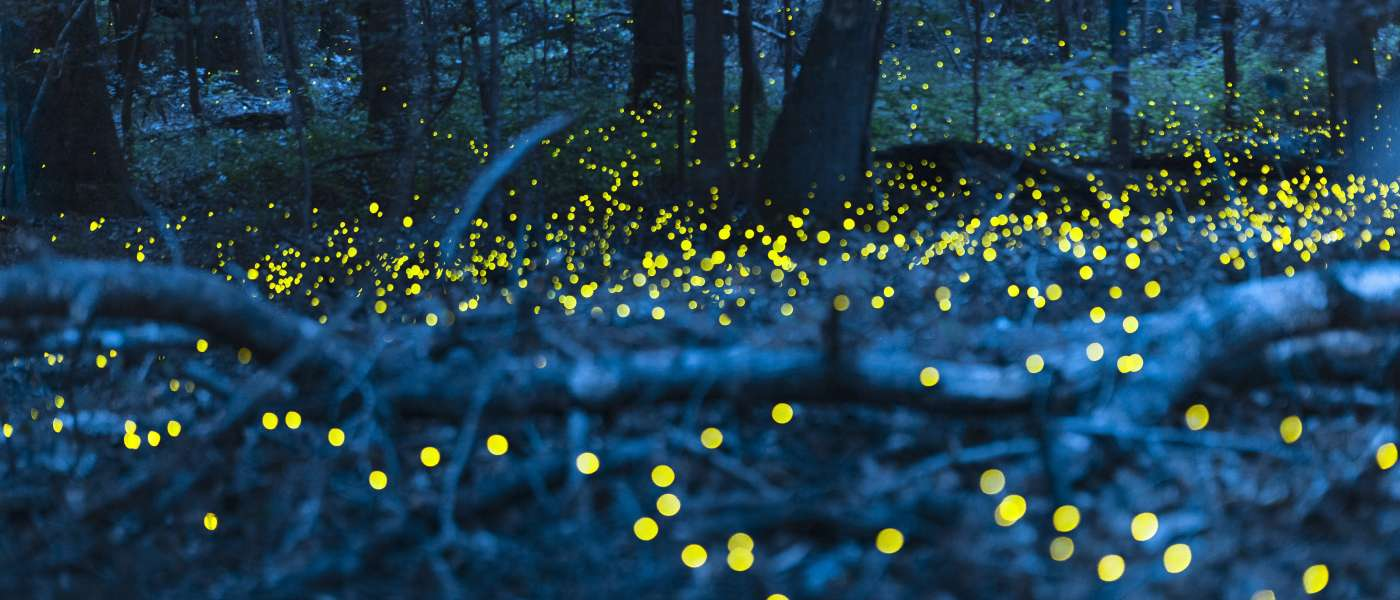
\includegraphics[width=0.9\linewidth]{Assets/Figures/synchronized_fireflies_phenomenon.jpg}
	\caption[Picture of fireflies flashing synchronously in a US National Park]{Synchronous fireflies at Congaree National Park, United States \cite{synched_fireflies_phenomenon}.}
	\label{fig:synched_fireflies_phenomenon}
\end{figure}

This phenomenon of fireflies synchronizing to each other has inspired scientists like Mirollo \& Strogatz \cite{mirollo_strogatz_PCO_synch} and in later time Kristian Nymoen et al. \cite{nymoen_synch}, to model and replicate this natural phenomenon in human-engineered systems. It turns out that this is not a biological, but mathematical, problem. Given the periodic and repeating nature of the flashing/firing of the fireflies, modelling a firefly has been done by looking at each firefly as a periodic signal or oscillator. This work \cite{mirollo_strogatz_PCO_synch, nymoen_synch} then ties into the broader work on synchronizing oscillators which has been subject to study for some time now []. What separates Mirollo-Strogatz and K. Nymoen's approaches from these other and previous oscillator-synchronizing methods, is mainly that here the oscillators are \textit{pulse-coupled} (which the fireflies also can be said to be), as opposed to the more ``standard'' and constraining \textit{phase-coupled} oscillators. Additionally, K. Nymoen's approach accounts for synchronizing initially heterogenous frequencies as well.

	\subsection{Multi-agent systems concepts}
	
	\begin{itemize}
		\item Stigmergy: meaning indirect communication and co-ordination by leaving traces of oneself in ones environment for others to observe or detect subsequently (kan diskuteres).
		\item Emergence
	\end{itemize}






% SECTION 3

\section{Oscillators and oscillator-synchronization}

	\gjor{Beskriv dette så godt at du kan snakke fritt om oscillatorers \textbf{faser} og \textbf{frekvenser} senere (i Implementation f.eks.), spesielt i tilfelle for noen ikke har vært borti det før, eller tatt et Signalbehandlings-kurs}
	
	\gjor{Skill på Pulse-coupled Oscillators, og Phase-coupled Oscillators}
	
	Teori og nyere cutting-edge/state-of-the-art metoder for fase-/frekvens-synkronisering i oscillatorer og liknende. Se Kristian Nymoens referanser i \cite{nymoen_synch} for eksempel. \nl
	
	\subsection{Phase and frequency}
	
	Much of the terminology from \cite{nymoen_synch} is used here. An oscillator $i$ is characterized by its \textit{phase} $\phi_i(t)$, which is—at the start of its periodic signal period—initialized to 0 and evolves towards 1 at a rate which is called the \textit{frequency} of the oscillator. So, in mathematical terms, the frequency $\omega_i(t)$ is then given by:
	
	\begin{equation}
	\label{phase_freq}
		\omega_i(t) = \frac{d \phi_i(t)}{d t} .
	\end{equation}

	When oscillator $i$'s phase is equal to 1 (i.e. when $\phi_i(t)=1$, or when the periodic signal period is over), we say oscillator $i$ has \textit{phase-climaxed}.
	
	An oscillator-period $T$ is defined as the inverse of the oscillator-frequency $\omega$. In mathematical terms:
	
	\begin{equation}
	\label{period_freq}
		T = 1/\omega .
	\end{equation}
	
	\subsection{Phase-adjustment}
	
	\gjor{Muligens inkluder introen i Section \ref{sec:phase_methods} her også (eller bare her?)}
	
	(Hvis relevante og ønskede) \nl
	Tidligere metoder til Fase-synkronisering i oscillatorer (puls- og/eller fase-koplede).
	
	% Mirollo-Strogatz's Phase-Adjustment
	\subsubsection{Mirollo-Strogatz's ``standard'' phase-adjustment} % used '-adjustment' before
	\label{mirollo_strogatz_phase_adjust}
	
	One approach having been used to achieve this in the past is Mirollo-Strogatz's ``Standard'' phase-adjustment in oscillators \cite{mirollo_strogatz_PCO_synch}.
	
	Each musical agent gets a new phase, $\phi(t^+) = P(\phi(t))$, accoring to the \textbf{phase update function \eqref{strog_phase}} upon perceiving a ``fire''-event from one of the other musical nodes:
	
	\begin{equation}
	\label{strog_phase}
		\phi(t^+) = P(\phi(t)) = (1 + \alpha)\phi(t)	,
	\end{equation}
	
	where ``\textit{$\alpha$ is the pulse coupling constant, denoting the strength between nodes}'' \cite{nymoen_synch}, $t^+$ denotes the time-step immediately after a ``fire''-event is heard, and $\phi(t)$ is the old frequency of the agent at time $t$. So, if e.g. $\alpha = 0.1$, then a musical agent's new and updated phase, immediately after hearing a ``fire''-signal from another agent, will be equal to $\phi(t^+) = P(\phi(t)) = (1 + 0.1)\phi(t) = 1.1\phi(t)$. 110\% of its old phase $\phi(t)$, that is. Hence, and in this way, the agent would be ``pushed'' to fire sooner than it would otherwise (as nodes fire once they have reached phase-climax $\phi(t)=1$).

	
	
	
	\subsection{Frequency-adjustment}
	
	\gjor{Muligens inkluder introen i Section \ref{sec:frequency_methods} her også (eller bare her?)}
	
	(If relevant and wanted) \nl
	Previous approaches to Frequency-synchronization in oscillators (pulse- and/or phase-coupled) [fixed\_freqs, fixed\_range\_freqs] where the oscillators's frequencies are either equal and fixed, or where frequencies are bound to initialize and stay within a fixed interval/range.
	
	
	% FREQ.-SYNCH APPROACH 1: LOW LEVEL Self-Awareness
	% Person X's "simpler" Frequency-Synchronization without any Self-Awareness components
	% Can use -updates or -synchronization
	\subsubsection{Person X's low SA-leveled frequency-adjustment}
	
	\gjor{Beskriv en simplere strategi/metode (to-be-implemented) for å oppnå harmonisk synkronitet i $\phi$- \& $\omega$-problemet (i.e. problemet der både faser og frekvenser starter med ulike og tilfeldige verdier, og altså begge trenger synkronisering) med frequency-adjustment, da uten noe Self-Awareness-egenskaper, hvis det finnes}
	
	
	

% SECTION 4

\section{Musical robots in music technology systems}

	M. J. Krzyzaniak and RITMO's musical robots, the Dr. Squiggles, have been used in various music technology systems previously \cite{dr_squiggles}. Corresponding 3D-models of these robots were designed by Pierre Potel \cite{pierre_potel} and will be reused, with permission, for the simulations in this thesis project.